\section{Технический проект}
\subsection{Общая характеристика организации решения задачи}

Необходимо спроектировать и разработать сайт, который должен способствовать продвижению компании на рынке.
Основной задачей системы является автоматизированная обработка изображений, загруженных пользователем из выбранной директории, с последующим применением набора предопределённых преобразований (аугментаций) и сохранением полученных результатов в отдельную директорию. Пользователь должен иметь возможность выбрать уровень интенсивности аугментации (низкий, средний, высокий), задать папку для сохранения и просматривать результаты преобразования в виде предварительного просмотра.
Обработка изображений осуществляется на стороне клиента, без необходимости подключения к сети Интернет. Это позволяет обеспечить максимальную независимость и приватность данных. Программа ориентирована на стабильную работу в среде Windows/Linux с минимальными системными требованиями и без фоновых сетевых процессов.

\subsection{Обоснование выбора технологий проектирования}

Используемые при разработке технологии отвечают современным стандартам и обеспечивают надёжность, удобство сопровождения и масштабируемость проекта. Для построения графического интерфейса выбрана кросс-платформенная библиотека PySide6, а для работы с изображениями — проверенная временем библиотека Pillow.

\subsubsection{Язык программирования Python}

Язык программирования Python был выбран как основной инструмент для реализации системы в силу следующих причин:

\begin{itemize}
	\item простота синтаксиса, позволяющая ускорить этапы разработки и отладки;
	\item широкая экосистема библиотек, включая Pillow для работы с изображениями и PySide6 для построения графического интерфейса;
	\item хорошая читаемость и расширяемость кода, что важно для последующего сопровождения проекта или его масштабирования;
	\item поддержка мультиплатформенности: программа может быть развёрнута как на Windows, так и на Linux, без необходимости значительных изменений в коде;
	\item активное сообщество и постоянное развитие языка и его инструментов.
\end{itemize}

Python используется как для создания пользовательского интерфейса, так и для реализации логики обработки изображений, что позволяет обеспечить целостность архитектуры и снизить сложность сопровождения программной системы.

\subsubsection{Исследование и выбор методов аугментации изображений}

Аугментация изображений (image augmentation) представляет собой процесс искусственного увеличения объема обучающей выборки путём внесения различных преобразований в исходные изображения. Актуальность применения аугментации особенно высока при работе с ограниченным числом изображений, в том числе для задач классификации, детекции и сегментации.

Цели внедрения аугментации в рамках настоящего программного решения:

\begin{itemize}
	\item увеличение разнообразия обучающей выборки без реального увеличения числа изображений;
	\item снижение переобучения алгоритмов машинного обучения при последующем применении данных;
	\item имитирование реальных условий съёмки, включая различия в освещении, положении камеры, шумовых помехах и т.д.;
	\item тестирование устойчивости алгоритмов распознавания и аналитики к искажениям;
	\item поддержка регуляризации и улучшение обобщающей способности обучаемых моделей.
\end{itemize}

%РИСУНОК
%Изображение сетка 2×3: оригинал и пять результатов (rotate, flip, noise, brightness, shift). 

Процесс отбора подходящих методов аугментации был организован в несколько этапов:

\begin{enumerate}
	\item Анализ имеющихся методов аугментации, реализуемых через библиотеки PIL, OpenCV и imgaug. Рассматривались следующие трансформации: геометрические (повороты, масштабирование, сдвиги, отражения), композиционные (обрезка, наложение).
	\item Формирование предварительного пула методов: поворот, шум (гауссовский, «соль и перец»), отражение, сдвиг, изменение яркости, обрезка, изменение контрастности.
	\item Применение методов к тестовой выборке (около 100 изображений), анализ визуальных изменений, а также оценка влияния на читаемость структуры изображения.
	\item Формализация критериев отбора: сохранение семантики изображения (разборчивость объектов), воспроизводимость и параметризация, реальная применимость к задачам распознавания и визуального анализа.
	\item Исключение методов, создающих риск искажения семантики (например, scale и агрессивный crop) или плохо применимых в условиях ограниченных вычислительных ресурсов.
\end{enumerate}

%таблица с видами аугментации

Таким образом, отбор прошли пять ключевых методов, которые соответствуют критериям качества, скорости и реалистичности: rotate, noise, flip, shift, brightness.

\subsubsection{Описание и исследование выбранных методов аугментации}

Для достижения наилучшего эффекта преобразования изображений были выбраны пять методов. В данном разделе проводится их подробный анализ, в том числе: принцип работы, исследованные диапазоны параметров, визуальные результаты и рекомендации по применению.

\begin{enumerate}
	\item Поворот изображения.

Поворот изображения на определённый угол позволяет имитировать изменение положения камеры или объекта. Преобразование сохраняет геометрию объектов и является одним из наименее деструктивных способов аугментации.

Пусть изображение задано в виде двемерной матрицы I(x, y) где, x, y принадлежит Z - координаты пикселей. Поворот изображения на угол в радианах вокруг центра ($x_c$, $y_c$) осуществляется по следующим формулам:


\[
\begin{bmatrix}
	x' \\
	y'
\end{bmatrix}
=
\begin{bmatrix}
	\cos\theta & -\sin\theta \\
	\sin\theta & \cos\theta
\end{bmatrix}
\cdot
\begin{bmatrix}
	x - x_c \\
	y - y_c
\end{bmatrix}
+
\begin{bmatrix}
	x_c \\
	y_c
\end{bmatrix}
\]

где $(x', y')$ — новые координаты пикселя после поворота. Угол $\theta$ считается положительным при повороте против часовой стрелки.

Диапазон параметров:
\begin{itemize}
	\item углы поворота: от -25 до +25 градусов;
	\item шаг исследуемых значений: 5 градусов.
\end{itemize}

Углы выше 30° приводят к искажению восприятия, особенно при наличии симметричных объектов. Было установлено, что диапазон ±25° обеспечивает визуальное разнообразие без потери информативности.

%ИЗОБРАЖЕНИЕ И ВАРИАНТЫ ПОВОРОТА -15 0 И 15 ГРАДУСОВ

	\item Добавление шума.
	
Добавление шумов позволяет имитировать условия плохой съёмки, передаёт реалистичность восприятия, особенно для задач, где необходимо устойчивое поведение к зашумлённым данным. Рассматривались два типа: гауссовский шум и соль и перец.

Гауссовский шум описывается добавлением случайной величины, распределённой по нормальному закону:

\[
I'(x, y) = I(x, y) + \mathcal{N}(0, \sigma^2),
\]
где $\mathcal{N}(0, \sigma^2)$ — нормально распределённая случайная величина со средним $0$ и дисперсией $\sigma^2$. Все значения выходного изображения ограничиваются диапазоном допустимых значений яркости (например, $[0, 255]$).
	
Шум типа «соль и перец» реализуется случайной заменой значения пикселей на минимальное (чёрное) или максимальное (белое) значение с заданной вероятностью $p$:

\[
I'(x, y) =
\begin{cases}
	0, & \text{с вероятностью } p/2 \\
	255, & \text{с вероятностью } p/2 \\
	I(x, y), & \text{с вероятностью } 1 - p
\end{cases}
\]


Диапазон параметров:
\begin{itemize}
	\item среднеквадратичное отклонение (гауссов шум): 2-25;
	\item соль и перец(процент испорченных пикселей): 0.01 - 0.10 (1-10\%).
\end{itemize}

При превышении указанных значений изображение становится трудноузнаваемым. Оптимальные значения были выбраны методом экспертной оценки и визуального тестирования.

%ИЗБОБРАЖЕНИЕ
% Примеры зашумления изображений с разной интенсивностью

	\item Отражение.
	
Отражение изображения по горизонтали или вертикали. Простой способ создания новых примеров без искажения формы. Отражение изображения по горизонтали или вертикали — это простая перестановка координат пикселей.


Горизонтальное отражение:

\[
I'(x, y) = I(W - 1 - x, y)
\]

где $W$ — ширина изображения.
	
Вертикальное отражение:

\[
I'(x, y) = I(x, H - 1 - y)
\]

где $H$ — высота изображения.


Обычно используется только горизонтальное отражение, так как вертикальное может нарушить семантику изображения (например, перевёрнутый текст или искажение направления объектов). 

%ИЗОБРАЖЕНИЕ оригинал и отраженное изображение

	\item Сдвиг.

Сдвиг изображения по горизонтали и вертикали, позволяющий сместить объект в пределах кадра, не нарушая общей структуры. 
Сдвиг изображения — это перемещение пикселей вдоль осей $X$ и/или $Y$ на заданное количество пикселей $\Delta x$ и $\Delta y$. При выходе за границы изображения пустые области заполняются фоновым значением (например, чёрным — 0).

\[
I'(x, y) =
\begin{cases}
	I(x - \Delta x, y - \Delta y), & \text{если } (x - \Delta x, y - \Delta y) \in \text{область изображения} \\
	0, & \text{иначе}
\end{cases}
\]

Сдвиги задаются как процент от размеров изображения:
\[
\Delta x = \alpha_x \cdot W,\quad \Delta y = \alpha_y \cdot H,\quad \alpha_x, \alpha_y \in [-0.15, 0.15]
\]

Диапазон параметров:

Смещение по X и Y: от -15\% до +15\% от размера изображения

Смещения более чем на 20\% влекут за собой обрезку ключевых областей. Оптимальные значения позволяют сохранить композицию при создании новой геометрии расположения объектов.

%ИЗОБРАЖЕНИЕ
%смещение по горзонтали +-10%


	\item Изменение яркости.

Изменение яркости изображения имитирует освещение в различных условиях (день, ночь, контровой свет и т.п.). Это особенно важно для универсализации восприятия моделей. Оно предполагает умножение значений всех пикселей изображения на коэффициент $\gamma \in [0.6, 1.4]$, где:

\begin{itemize}
	\item $\gamma < 1$ — затемнение изображения;
	\item $\gamma > 1$ — увеличение яркости.
\end{itemize}

\[
I'(x, y) = \text{clip}\left( \gamma \cdot I(x, y),\ 0,\ 255 \right)
\]

Диапазон параметров: коэффициент изменения яркости: 0.6 – 1.4
(где 1.0 — исходное значение)

Значения ниже 0.5 делают изображение почти чёрным, выше 1.5 — засвеченным. Оптимальный диапазон обеспечивает баланс между реализмом и информативностью.

% ИЗОБРАЖЕНИЕ
% зимененение яркости 0.6, 1.0, 1.4

\end{enumerate}

%таблица выбранных оптимальных значений

\subsubsection{Оценка вычислительной сложности методов аугментации}

Для обеспечения эффективной работы системы на устройствах с ограниченными вычислительными ресурсами была проведена оценка сложности выбранных методов аугментации. 

\begin{enumerate}
	\item Поворот: Сложность поворота изображения определяется необходимостью пересчета координат каждого пикселя с использованием матрицы поворота. Для изображения размером $W \times H$ сложность составляет $O(W \cdot H)$, что приемлемо для большинства современных устройств.
	\item Добавление шума: Генерация гауссовского шума или шума "соль и перец" требует прохода по всем пикселям изображения, что также дает сложность $O(W \cdot H)$. Однако генерация случайных чисел может добавить небольшую накладную стоимость.
	\item Отражение: Операция отражения (по горизонтали или вертикали) сводится к перестановке пикселей, что выполняется за $O(W \cdot H)$.
	\item Сдвиг: Сдвиг изображения также требует прохода по всем пикселям, сложность составляет $O(W \cdot H)$. Дополнительные затраты могут возникнуть при заполнении пустых областей.
	\item Изменение яркости: Умножение значений пикселей на коэффициент $\gamma$ выполняется за один проход по изображению, что дает сложность $O(W \cdot H)$.
\end{enumerate}

Все методы имеют линейную сложность $O(W \cdot H)$, что делает их подходящими для обработки изображений в реальном времени на стандартных устройствах. Однако при пакетной обработке больших объемов данных (например, 100 изображений размером 500×500 пикселей) рекомендуется использовать многопоточность для повышения производительности.

\subsubsection{Конфигурация уровней аугментации и автоматизация параметров}

Для повышения гибкости и упрощения взаимодействия с системой аугментации в пользовательском интерфейсе были реализованы три уровня интенсивности преобразований: low, medium и high. Каждый уровень соответствует предопределённому набору параметров, автоматически применяемых к каждому изображению.

\textbf{Обоснование уровней}

Уровни были выделены на основе эмпирического анализа, где оценивалась степень трансформации и её влияние на восприятие изображения. % На таблице ниже представлены сводные настройки для каждого уровня
\begin{itemize}
	\item low - отражение, яркость;
	\item medium - отражение, яркость, поворот, шум;
	\item high - отражение, яркость, поворот, шум, сдвиг.
\end{itemize}
	
%ИЗОБРАЖЕНИЕ
%Сравнение изображений при применении уровней low, medium, high.

Система построена по принципу передачи параметров через уровень аугментации. Пользователь выбирает нужный уровень в интерфейсе, и далее программа сопоставляет уровень с конфигурацией (словарь параметров), применяет соответствующие методы аугментации, обеспечивает единообразное поведение для всех изображений партии. Выделение уровней аугментации: упрощает пользовательский опыт, обеспечивает стабильность качества результатов и позволяет масштабировать систему без изменений в логике преобразований.

Для обоснования применимости выбранных методов аугментации и их параметров была проведена оценка качества сгенерированных изображений по следующим критериям:
\begin{itemize}
	\item визуальная читаемость изображения (отсутствие чрезмерных искажений);
	\item сохранение признаков исходного объекта (не теряются ключевые контуры, формы, текстуры);
	\item разнообразие выборки (каждая аугментация должна вносить полезную вариативность, а не избыточный шум);
	\item устойчивость к переобучению на основе опыта использования в системах распознавания (принцип увеличения генерализации).
\end{itemize}

На основании анализа параметров можно выделить следующие оптимальные значения:

\begin{itemize}
	\item поворот: +-15 градусов (максимум 25 градусов);
	\item гауссов шум: 10-15;
	\item соль/Перец: 3-5\%;
	\item яркость: от 0.8 до 1.2;
	\item до 10\% по X и Y;
	\item горизонтальное.
\end{itemize}

\subsection{Проектирование пользовательского интерфейса}

На основании требований к пользовательскому интерфейсу, представ
ленных в пункте 2.3, был разработан графический интерфейс программной
системы.

На рисунке 3.1 представлен макет интерфейса приложения. Макет содержит следующие элементы:

\begin{enumerate}
	\item Поле, содержащее окна для отображения примера исходного изображения и аугментированного.
	\item Кнопка выбора папки с изображениями для аугментации.
	\item Поле, содержащее выпадающий список с параметрами аугментации.
	\item Кнопка выбора папки, в которую необходимо сохранить аугментированные изображения.
	\item Кнопка запуска процесса аугментации.
	\item Кнопка для открытия папки с аугментированными изображениями.
	\item Поле, содержащее аугментированные изображения.
	\item Кнопка настройки аугментации.
	\item Шкала прогресса завершения агументации.
\end{enumerate}


\begin{figure}
	\centering
	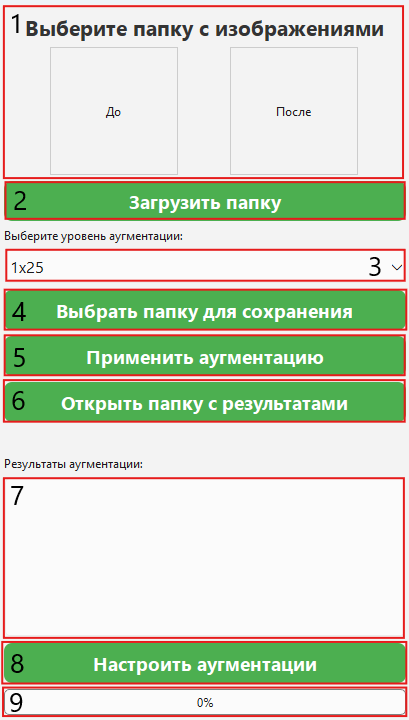
\includegraphics[width=0.4\linewidth]{images/interfacenum}
	\caption{Макет интерфейса приложения}
	\label{fig:interfacenum}
\end{figure}
